% =====================================================================
%  NATURAL SCIENCES TRIPOS  -  PART II PHYSICS
%  ADVANCED AND QUANTUM OPTICS  -  Examiners' Solutions / Mark Scheme
%
%  Compile with pdflatex.
% =====================================================================
\documentclass[11pt]{article}

\usepackage[a4paper,top=2.3cm,bottom=2.3cm,left=2.5cm,right=2.5cm]{geometry}
\usepackage{amsmath,amssymb}
\usepackage{graphicx}
\usepackage{tikz}
\usepackage{enumitem}
\usepackage{fancyhdr}
\usepackage{mathptmx}
\usepackage{xcolor}

\setlength{\parindent}{0pt}
\setlength{\parskip}{6pt}

% Marks in the right margin -------------------------------------------
\newcommand{\qmarks}[1]{\hfill\makebox[0pt][r]{\hspace{1.5em}\textbf{[#1]}}}

% Question numbering --------------------------------------------------
\newcounter{question}
\newcommand{\question}{\par\vspace{6pt}\refstepcounter{question}%
  \noindent{\large\textbf{Question \thequestion}}\par\vspace{2pt}}

% Part labelling ------------------------------------------------------
\newlist{parts}{enumerate}{1}
\setlist[parts]{label=(\alph*),leftmargin=2.2em,labelsep=0.6em,
                itemsep=6pt,topsep=4pt}

% Marker's notes ------------------------------------------------------
\newcommand{\note}[1]{\par\vspace{2pt}{\small\textit{Marker's note: #1}}\par}

\pagestyle{fancy}
\fancyhf{}
\rhead{\small AQO 2026 --- Solutions}
\lhead{\small Part II Physics}
\cfoot{\thepage}
\renewcommand{\headrulewidth}{0.4pt}

\newcommand{\sectionbanner}[1]{%
  \vspace{8pt}\noindent{\large\textbf{#1}}\par\vspace{2pt}\hrule\vspace{6pt}}

\begin{document}

% =====================================================================
%  TITLE
% =====================================================================
\begin{center}
{\large\textbf{NATURAL SCIENCES TRIPOS \quad Part II Physics}}\\[4pt]
{\large\textbf{ADVANCED AND QUANTUM OPTICS}}\\[6pt]
{\textbf{Examiners' Solutions and Mark Scheme}}\\[2pt]
Wednesday 10th June 2026
\end{center}

\vspace{4pt}
\noindent
\textit{Total marks: 56 ($4\times4$ in Section A, $2\times20$ in Section B).
Marks shown in square brackets in the right margin. Method marks are awarded
for a correct approach even where the final number is wrong; alternative valid
derivations should be credited fully.}

\hrule

% =====================================================================
%  SECTION A
% =====================================================================
\sectionbanner{SECTION A}

% ----------------------------- Q1 ------------------------------------
\question
\textit{Gaussian beam collimation.}

The Rayleigh range $z_0$ is the axial distance from the waist over which the
beam cross-sectional area doubles; equivalently it is the distance at which the
beam radius has grown to $\sqrt{2}\,W_0$, and the distance at which the
wavefront curvature is most pronounced. It is given by
\[
  z_0 = \frac{\pi W_0^{2}}{\lambda}.
\]
\qmarks{1}

Numerically, with $W_0 = 5.0\times10^{-4}$~m and
$\lambda = 1.0\times10^{-6}$~m,
\[
  z_0 = \frac{\pi (5.0\times10^{-4})^{2}}{1.0\times10^{-6}}
      = \frac{\pi \times 2.5\times10^{-7}}{1.0\times10^{-6}}
      \approx 0.785\ \text{m}.
\]
\qmarks{1}

At $z = 20$~m we have $z \gg z_0$, so the beam is in the far field and
\[
  W(z) = W_0\sqrt{1+(z/z_0)^{2}} \approx W_0\frac{z}{z_0}
       = 5.0\times10^{-4}\times\frac{20}{0.785}
       \approx 1.27\times10^{-2}\ \text{m}.
\]
The beam diameter is therefore $2W(z) \approx 2.5$~cm.
\qmarks{1}

A larger waist gives a larger Rayleigh range ($z_0 \propto W_0^{2}$) and a
smaller far-field divergence half-angle $\theta_0 = \lambda/(\pi W_0)$. The
beam therefore stays collimated over a longer distance; physically, a wider
beam has a smaller spread of transverse wavevectors and so diffracts less.
\qmarks{1}

\note{Accept $z_0$ defined either via the area doubling or the
$\sqrt2\,W_0$ radius. Full far-field credit if the student uses the exact
$W(z)$ expression and obtains $\approx 1.27$~cm radius. The final comment must
link $W_0$ to either $z_0$ or $\theta_0$.}

% ----------------------------- Q2 ------------------------------------
\question
\textit{Second-order nonlinear processes.}

For a single field $E(t) = E\cos(\omega t)$ in a medium with a second-order
nonlinearity, the nonlinear polarisation is
$P^{(2)} \propto E^{2}\cos^{2}(\omega t)
 = \tfrac12 E^{2}\,[\,1 + \cos(2\omega t)\,]$.
The $\cos(2\omega t)$ term is an oscillating polarisation at twice the input
frequency, which radiates a field at $2\omega$: this is \textbf{second-harmonic
generation (frequency doubling)}. The constant term is a static (d.c.)
polarisation proportional to the optical intensity: this is \textbf{optical
rectification}.
\qmarks{2}

These processes require a non-zero $\chi^{(2)}$, which is possible only in a
\textbf{non-centrosymmetric} crystal (a material lacking inversion symmetry).
\qmarks{1}

In a centrosymmetric medium, inverting the applied field
$E \to -E$ must invert the polarisation, $P \to -P$. But a $\chi^{(2)}E^{2}$
term is even in $E$ and so is unchanged under $E\to -E$; consistency therefore
forces $\chi^{(2)} = 0$. Equivalently, the anharmonic potential of a
centrosymmetric medium has no cubic ($x^{3}$) term.
\qmarks{1}

\note{The symmetry argument (parity of $P$ under $E\to-E$) is the key point;
accept the equivalent statement about the cubic term in the Lorentz potential.}

% ----------------------------- Q3 ------------------------------------
\question
\textit{Symmetric two-mirror resonator stability.}

For a two-mirror resonator the round-trip ray-transfer matrix gives the
stability (confinement) condition
\[
  0 \le \Bigl(1+\frac{d}{R_1}\Bigr)\Bigl(1+\frac{d}{R_2}\Bigr) \le 1,
  \qquad\text{i.e.}\qquad 0 \le g_1 g_2 \le 1 .
\]
For a symmetric resonator $R_1 = R_2 = R$, so $g_1 = g_2 = g = 1 + d/R$ and the
condition becomes $g^{2}\le 1$, i.e.
\[
  -1 \le 1+\frac{d}{R} \le 1
  \qquad\Longrightarrow\qquad
  0 \le \frac{d}{|R|} \le 2 ,
\]
where concave mirrors ($R<0$) are required.
\qmarks{2}

The three special configurations are:
\[
  \frac{d}{|R|} = 0 \ \text{(planar)},\quad
  \frac{d}{|R|} = 1 \ \text{(confocal)},\quad
  \frac{d}{|R|} = 2 \ \text{(concentric)} .
\]
\qmarks{1}

The \textbf{confocal} resonator, $d/|R| = 1$, lies at the centre of the stable
range and is the most robust against misalignment. The planar and concentric
configurations sit exactly on the stability boundary ($g_1g_2 = 1$ or $0$), so
any small perturbation of mirror tilt or spacing pushes them out of the stable
region and rays walk off; the confocal resonator is maximally far from these
edges.
\qmarks{1}

\note{Derivation of $0\le g_1g_2\le1$ may be quoted from lectures; the
specialisation to the symmetric case and the identification of the three points
are required. The robustness argument must refer to confocal being in the
middle / planar and concentric being on the boundary.}

% ----------------------------- Q4 ------------------------------------
\question
\textit{Resonantly driven two-level atom.}

\textbf{(i) No spontaneous emission.} Solving the resonant ($\Delta=0$)
two-level equations with the atom initially in the ground state gives
$|c_e(t)|^{2} = \sin^{2}(\Omega_0 t/2) = \tfrac12[1-\cos(\Omega_0 t)]$.
The excited-state population oscillates undamped between $0$ and $1$ at the
Rabi frequency $\Omega_0$ --- \emph{Rabi oscillations}. At long times it
continues to oscillate; there is no steady state.
\qmarks{2}

\textbf{(ii) With spontaneous emission $\gamma\approx0.2\,\Omega_0$.} The
optical Bloch equations now include damping. The population still oscillates
initially, but the oscillations are damped and the system relaxes to a steady
state with $0 < \rho_{ee} < \tfrac12$.
\qmarks{1}

\begin{center}
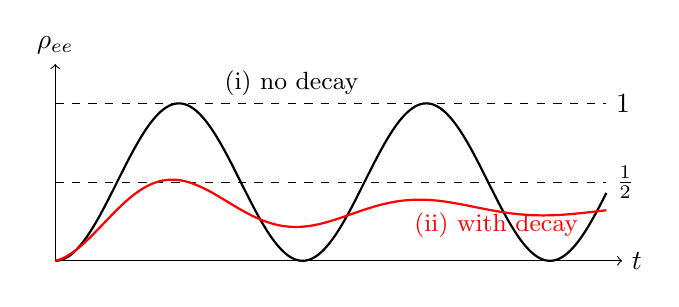
\begin{tikzpicture}[scale=1.0]
% axes
\draw[->] (0,0) -- (7.2,0) node[right]{$t$};
\draw[->] (0,0) -- (0,2.5) node[above]{$\rho_{ee}$};
\draw[dashed] (0,2.0) -- (7.0,2.0) node[right]{$1$};
\draw[dashed] (0,1.0) -- (7.0,1.0) node[right]{$\tfrac12$};
% (i) undamped: full-amplitude sinusoid 0..1
\draw[thick,domain=0:7,samples=200,smooth]
  plot (\x,{1.0 - 1.0*cos(deg(2*\x))});
\node at (3.0,2.25) {\small (i) no decay};
% (ii) damped, settling below 1/2
\draw[thick,red,domain=0:7,samples=200,smooth]
  plot (\x,{0.65 - 0.65*exp(-0.35*\x)*cos(deg(2*\x))});
\node[red] at (5.6,0.45) {\small (ii) with decay};
\end{tikzpicture}
\end{center}

Physically, in case (i) the dynamics is fully coherent and energy is
periodically exchanged between the atom and the field. In case (ii) each
spontaneous-emission event randomises the atomic phase and destroys the
coherence; after a few cycles the oscillation washes out and the atom reaches a
balance between coherent driving and incoherent decay --- the steady state.
\qmarks{1}

\note{Sketches need not be analytically exact: award the marks for
(i) a full-amplitude undamped oscillation reaching $1$, and (ii) a damped
oscillation settling to a constant value strictly below $\tfrac12$. The
explanation must mention loss of coherence / approach to steady state.}

% =====================================================================
%  SECTION B
% =====================================================================
\sectionbanner{SECTION B}

% ----------------------------- Q5 ------------------------------------
\question
\textit{Optical coherence and coherence-gated imaging.}

\begin{parts}

\item The coherence time is the characteristic ``memory time'' of the field
fluctuations, defined through the power-equivalent width of the normalised
temporal coherence,
\[
  \tau_c = \int_{-\infty}^{\infty} |g(\tau)|^{2}\,d\tau .
\]
The coherence length is the corresponding propagation distance,
$\ell_c = c\,\tau_c$. The spectral width is the reciprocal of the coherence
time,
\[
  \Delta\nu_c = \frac{1}{\tau_c}.
\]
\qmarks{3}

\note{Award 1 mark each for $\tau_c$ (definition or words), $\ell_c=c\tau_c$,
and $\Delta\nu_c = 1/\tau_c$.}

\item Writing the two recombining fields as $U_1 = U(t)$ and
$U_2 = U(t+\tau)$, both of intensity $I_0$, the detected intensity is
\[
  I = \langle|U_1+U_2|^{2}\rangle
    = I_0 + I_0 + 2\,\mathrm{Re}\langle U^{*}(t)U(t+\tau)\rangle
    = 2I_0\bigl[1 + \mathrm{Re}\{g(\tau)\}\bigr],
\]
using $g(\tau) = \langle U^{*}(t)U(t+\tau)\rangle/I_0$. Writing
$g(\tau) = |g(\tau)|\,e^{j\varphi(\tau)}$ gives
\[
  \boxed{\,I(\tau) = 2I_0\bigl[\,1 + |g(\tau)|\cos\varphi(\tau)\,\bigr]\,},
  \qquad \varphi(\tau) = \arg\{g(\tau)\}.
\]
\qmarks{2}

For a perfectly monochromatic wave $|g(\tau)| = 1$ for all $\tau$, so
$I(\tau)$ is a pure cosine of constant unit visibility. For a
quasi-monochromatic wave $|g(\tau)| = |g_a(\tau)|$ decays over $\sim\tau_c$, so
the fringes have a cosine carrier under an envelope $|g_a(\tau)|$ that decays
away from $\tau = 0$: the visibility falls to zero for $|\tau| \gg \tau_c$.
The envelope of the interferogram therefore directly gives $|g(\tau)|$
(and the fringe positions give $\varphi(\tau)$).
\qmarks{3}

\begin{center}
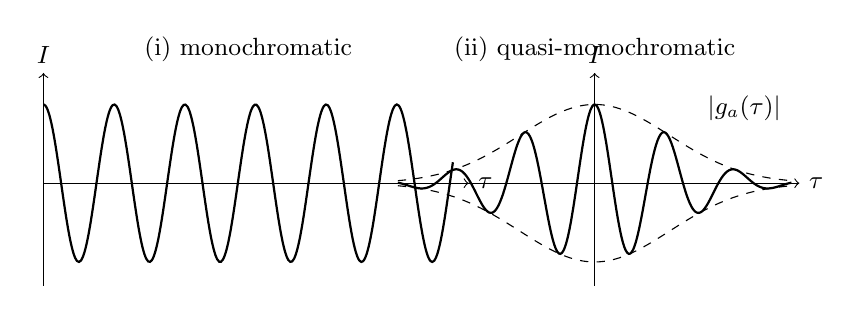
\begin{tikzpicture}[scale=1.0]
% (i) monochromatic
\begin{scope}
\draw[->] (0,0) -- (5.4,0) node[right]{\small $\tau$};
\draw[->] (0,-1.3) -- (0,1.4) node[above]{\small $I$};
\draw[thick,domain=0:5.2,samples=220,smooth] plot (\x,{cos(deg(7*\x))});
\node at (2.6,1.7) {\small (i) monochromatic};
\end{scope}
% (ii) quasi-monochromatic
\begin{scope}[xshift=7.0cm]
\draw[->] (-2.6,0) -- (2.6,0) node[right]{\small $\tau$};
\draw[->] (0,-1.3) -- (0,1.4) node[above]{\small $I$};
\draw[thick,domain=-2.5:2.5,samples=260,smooth]
  plot (\x,{exp(-0.55*\x*\x)*cos(deg(7*\x))});
\draw[dashed,domain=-2.5:2.5,samples=120,smooth]
  plot (\x,{exp(-0.55*\x*\x)});
\draw[dashed,domain=-2.5:2.5,samples=120,smooth]
  plot (\x,{-exp(-0.55*\x*\x)});
\node at (0,1.7) {\small (ii) quasi-monochromatic};
\node at (1.9,0.95) {\small $|g_a(\tau)|$};
\end{scope}
\end{tikzpicture}
\end{center}

\note{The derivation (3 lines) earns 2 marks. The two annotated sketches:
1 mark for the constant-visibility cosine, 1 mark for the decaying envelope,
1 mark for stating that the envelope yields $|g(\tau)|$.}

\item The coherence length of a source of centre wavelength $\lambda_0$ and
spectral width $\Delta\lambda$ is, to within a numerical factor of order unity,
\[
  \ell_c \sim \frac{\lambda_0^{2}}{\Delta\lambda}
        = \frac{(800\times10^{-9})^{2}}{25\times10^{-9}}
        = \frac{6.4\times10^{-13}}{2.5\times10^{-8}}
        \approx 2.6\times10^{-5}\ \text{m}
        \approx 26\ \mu\text{m}.
\]
\qmarks{2}

A short coherence length is desirable because interference fringes appear only
when the two arms are matched to within $\sim\ell_c$. The fringe burst from a
given reflecting boundary is therefore localised to a narrow range of delay,
giving good axial (depth) discrimination and allowing closely spaced layers to
be separated --- this is \emph{coherence gating}.
\qmarks{2}

\note{Accept $\ell_c$ in the range $\sim10$--$30\ \mu$m depending on the
numerical factor used; full marks for $\lambda_0^2/\Delta\lambda$ with correct
arithmetic. The explanation must connect short $\ell_c$ to depth localisation.}

\item Each boundary $i$ reflects a fraction $r_i$ of the field with its own
delay $\tau_i$. The interferogram contains terms $\propto r_i\,
|g_a(\tau-\tau_i)|\cos[\omega_0(\tau-\tau_i)+\phi_a]$. Because $|g_a|$ is narrow
(width $\tau_c$), interference fringes appear only when the scanned reference
delay $\tau$ matches $\tau_i$ to within $\tau_c$. Each boundary therefore
generates a separate, well-localised fringe burst centred on its own $\tau_i$.
\qmarks{2}

The axial separation of two layers is obtained from the difference in the delay
positions of their bursts: a delay difference $\Delta\tau$ corresponds to an
optical path difference $c\,\Delta\tau$, hence a physical layer separation
$\Delta z = c\,\Delta\tau/(2n)$ (the factor of two for the round trip, $n$ the
sample refractive index).
\qmarks{2}

\note{1 mark for ``fringes only when $\tau\approx\tau_i$''; 1 mark for distinct
bursts per boundary; 2 marks for converting the burst-position difference into
a physical depth (factor of 2 for round trip expected, but do not penalise
heavily if omitted).}

\item The axial resolution is set by the coherence length of the source,
$\Delta z \approx \ell_c/(2n) \sim \lambda_0^{2}/(n\,\Delta\lambda)$, which
depends only on the optical \emph{spectrum} of the source and not on the
focusing geometry. By contrast, in a conventional microscope the axial
resolution comes from the depth of field of the focused spot and so scales with
the numerical aperture. In OCT the depth information is encoded in the
\emph{time delay}, decoupling it from the transverse focusing; hence the axial
resolution is independent of NA (only the lateral resolution depends on NA).
\qmarks{4}

\note{Full marks for clearly stating that OCT axial resolution is fixed by the
source spectrum / coherence length whereas microscope axial resolution is fixed
by NA-dependent depth of field, with the reason being that depth is encoded in
delay. Partial credit (2) for stating the result without the reasoning.}

\end{parts}

% ----------------------------- Q6 ------------------------------------
\question
\textit{The quantised single-mode field and its states.}

\begin{parts}

\item Since $\hat{a}|n\rangle = \sqrt{n}\,|n-1\rangle$ and
$\hat{a}^{\dagger}|n\rangle = \sqrt{n+1}\,|n+1\rangle$, both terms in
$\hat{E}_x \propto \hat{a}+\hat{a}^{\dagger}$ change the photon number by one,
so they map $|n\rangle$ onto states orthogonal to $|n\rangle$:
\[
  \langle n|\hat{E}_x|n\rangle
  \propto \langle n|(\hat{a}+\hat{a}^{\dagger})|n\rangle
  = \sqrt{n}\,\langle n|n-1\rangle + \sqrt{n+1}\,\langle n|n+1\rangle = 0 .
\]
\qmarks{2}

For the second moment, with $\hat{E}_x = \mathcal{E}_0(\hat a+\hat a^\dagger)$,
\[
  \hat{E}_x^{2} = \mathcal{E}_0^{2}
   \bigl(\hat a^{2} + \hat a^{\dagger 2}
        + \hat a^{\dagger}\hat a + \hat a\hat a^{\dagger}\bigr).
\]
The $\hat a^{2}$ and $\hat a^{\dagger 2}$ terms have zero diagonal matrix
element. Using $\hat a\hat a^{\dagger} = \hat a^{\dagger}\hat a + 1$,
\[
  \langle n|\hat{E}_x^{2}|n\rangle
  = \mathcal{E}_0^{2}\,\langle n|(2\hat a^{\dagger}\hat a + 1)|n\rangle
  = 2\mathcal{E}_0^{2}\Bigl(n+\tfrac12\Bigr) \;\propto\; \Bigl(n+\tfrac12\Bigr).
\]
\qmarks{2}

A classical field has a well-defined oscillating amplitude, i.e.
$\langle\hat{E}_x\rangle\neq0$. A Fock state has $\langle\hat{E}_x\rangle = 0$
for every $n$, no matter how large, even though
$\langle\hat{E}_x^{2}\rangle\neq0$. The field has a definite ``energy'' but a
completely random phase, so a Fock state does not resemble a classical
monochromatic wave.
\qmarks{1}

\note{2 marks for $\langle\hat E_x\rangle=0$ with the orthogonality argument;
2 marks for $\langle\hat E_x^2\rangle\propto(n+\tfrac12)$ using the commutator;
1 mark for the physical comment about random phase.}

\item The probability of finding $n$ photons is
\[
  P_n = |\langle n|\alpha\rangle|^{2}
      = \left|e^{-|\alpha|^{2}/2}\frac{\alpha^{n}}{\sqrt{n!}}\right|^{2}
      = e^{-|\alpha|^{2}}\frac{|\alpha|^{2n}}{n!},
\]
which is a Poisson distribution with parameter $|\alpha|^{2}$.
\qmarks{2}

The mean photon number is
\[
  \bar{n} = \langle\alpha|\hat a^{\dagger}\hat a|\alpha\rangle
          = \langle\alpha|\,\alpha^{*}\alpha\,|\alpha\rangle
          = |\alpha|^{2}.
\]
\qmarks{1}

For the variance, use
$\hat a^{\dagger}\hat a\hat a^{\dagger}\hat a
 = \hat a^{\dagger}(\hat a^{\dagger}\hat a + 1)\hat a
 = \hat a^{\dagger 2}\hat a^{2} + \hat a^{\dagger}\hat a$, so
\[
  \langle\hat n^{2}\rangle
  = \langle\alpha|\hat a^{\dagger 2}\hat a^{2}|\alpha\rangle
   + \langle\alpha|\hat a^{\dagger}\hat a|\alpha\rangle
  = |\alpha|^{4} + |\alpha|^{2} = \bar n^{2} + \bar n,
\]
hence
\[
  (\Delta n)^{2} = \langle\hat n^{2}\rangle - \bar n^{2} = \bar n .
\]
This is the defining signature of a Poisson distribution.
\qmarks{2}

\note{2 marks for showing $P_n$ is Poissonian; 1 mark for $\bar n=|\alpha|^2$;
2 marks for $(\Delta n)^2=\bar n$ via the normal-ordering step. Accept quoting
the variance of a Poisson distribution \emph{provided} $P_n$ was first shown to
be Poissonian.}

\item Because $\hat a|\alpha\rangle = \alpha|\alpha\rangle$ and
$\langle\alpha|\hat a^{\dagger} = \alpha^{*}\langle\alpha|$, the field
expectation value is non-zero:
$\langle\alpha|(\hat a+\hat a^{\dagger})|\alpha\rangle
 = \alpha + \alpha^{*} = 2\,\mathrm{Re}(\alpha)\neq0$.
A coherent state is a superposition of many number states, so the
amplitude-changing operators no longer give zero --- it has a well-defined mean
field with a definite phase.
\qmarks{2}

The fractional uncertainty in photon number is
\[
  \frac{\Delta n}{\bar n} = \frac{\sqrt{\bar n}}{\bar n}
                          = \frac{1}{\sqrt{\bar n}}
                          = \frac{1}{|\alpha|} \;\to\; 0
  \quad\text{as } |\alpha|\to\infty .
\]
\qmarks{1}

Thus for large $|\alpha|$ a coherent state has both a vanishing relative
intensity uncertainty and a well-defined phase, approaching a classical
monochromatic wave of fixed amplitude and phase --- exactly the idealised
output of a laser well above threshold.
\qmarks{1}

\note{2 marks for the non-zero mean field with reasoning; 1 mark for
$\Delta n/\bar n = 1/|\alpha|\to0$; 1 mark for the link to the classical /
laser limit.}

\item Acting on the input $|0\rangle_{0}|1\rangle_{1}
= \hat a^{\dagger}_{1}|0\rangle_{0}|0\rangle_{1}$ with the given relation,
\[
  |0\rangle_{0}|1\rangle_{1}
  = \hat a^{\dagger}_{1}|0\rangle
  = \frac{1}{\sqrt2}\bigl(i\,\hat a^{\dagger}_{2}
       + \hat a^{\dagger}_{3}\bigr)|0\rangle
  = \frac{1}{\sqrt2}\bigl(i\,|1\rangle_{2}|0\rangle_{3}
       + |0\rangle_{2}|1\rangle_{3}\bigr).
\]
The photon emerges in an entangled superposition of the two output ports, with
a 50:50 probability of being detected in either.
\qmarks{2}

The beam-splitter transformation cannot be written consistently using only the
populated input mode: the vacuum mode $\hat a_{0}$ must appear so that the
output operators obey the correct commutation relations. Physically, the
\emph{vacuum fluctuations} entering the unused port are essential and influence
the quantum statistics of the output.
\qmarks{1}

\note{2 marks for the correct entangled output state; 1 mark for the role of
the vacuum port (commutation relations / vacuum fluctuations).}

\item In a coincidence measurement \emph{no} coincidences are observed: the two
indistinguishable photons always leave together from the same output port
(the output state is $\tfrac{i}{\sqrt2}(|2\rangle_2|0\rangle_3
+|0\rangle_2|2\rangle_3)$). This is the Hong--Ou--Mandel effect, arising from
destructive interference of the two ``both-transmitted'' and
``both-reflected'' amplitudes.
\qmarks{2}

By introducing a variable relative delay $\tau$ between the two photons (e.g.\
with a delay line) and recording the coincidence rate, one observes a dip --- 
the ``HOM dip'' --- that reaches zero at $\tau = 0$ and rises as the photons
are made distinguishable. The depth and width of the dip quantify the
indistinguishability of the photon pair.
\qmarks{1}

\note{2 marks for ``photons leave together / coincidences vanish'' with a brief
justification (interference of amplitudes). 1 mark for describing the HOM dip
as a function of delay as the test of indistinguishability.}

\end{parts}

\vspace{1.0cm}
\hrule
\vspace{4pt}
{\small\textit{End of solutions. Section A: 16 marks. Section B: 40 marks.
Paper total: 56 marks.}}

\end{document}
